\section{Analyse}

Dieses Kapitel analysiert die bestehende Situation im Budget-Controlling und definiert die Anforderungen an die zu entwickelnde Middleware. Die Analyse folgt einem strukturierten Vorgehen: Zunächst wird der Ist-Zustand erfasst, anschließend werden funktionale und nicht-funktionale Anforderungen abgeleitet \citep{sommerville2015}.

\subsection{Ist-Analyse}

\subsubsection{Excel-basierter Workflow}

Der aktuelle Workflow basiert auf einer zentralen Excel-Datei (\texttt{Budgetcontrolling.xlsx}), die über SharePoint geteilt wird. Die Datei integriert Daten aus verschiedenen Quellen mittels Power Query.

\begin{table}[H]
\centering
\caption{Sheets in Budgetcontrolling.xlsx}
\label{tab:excel-sheets}
\begin{tabularx}{\textwidth}{lXl}
\toprule
\textbf{Sheet} & \textbf{Zweck} & \textbf{Quelle} \\
\midrule
qry\_CALM\_Data & User Stories mit \gls{psp}-Zuordnung & Power Query \\
CADO & Zeitbuchungen (Ist-Stunden) & SAP-Export \\
PSP-Elemente & Budget pro \gls{psp} & Manuell \\
1. PSP-Zuordnung & Manuelle Zuordnungen & Manuell \\
2. PSP-Zuordnung & Fallback: Team $\rightarrow$ Timebox $\rightarrow$ \gls{psp} & Manuell \\
Reporting & Zusammenfassung pro Team & Berechnet \\
\bottomrule
\end{tabularx}
\end{table}

\subsubsection{Budget-Metriken}

Die folgenden Metriken werden für das Budget-Controlling verwendet. Diese Kennzahlen entsprechen den im Projektmanagement etablierten Earned Value Management (EVM) Metriken \citep{kerzner2017, pmi2021}:

\begin{table}[H]
\centering
\caption{Budget-Metriken und ihre Berechnung}
\label{tab:metriken}
\begin{tabularx}{\textwidth}{lXl}
\toprule
\textbf{Metrik} & \textbf{Beschreibung} & \textbf{Berechnung} \\
\midrule
Budget & Geplantes Budget & Summe aus PSP-Elemente \\
Actual & Bereits geleistete Arbeit & CADO Stunden / 8 \\
\gls{etc} & Noch zu leistende Arbeit & qry\_CALM\_Data (mit \gls{psp}) \\
\gls{eac} & Geschätzte Gesamtkosten & Actual + \gls{etc} \\
\bottomrule
\end{tabularx}
\end{table}

\subsubsection{Problemanalyse}

Die Analyse des bestehenden Workflows zeigt folgende Probleme:

\begin{enumerate}
    \item \textbf{Keine Echtzeitdaten}: Power Query wird nur bei manuellem Refresh aktualisiert
    \item \textbf{Keine API}: Andere Systeme können nicht auf die Daten zugreifen
    \item \textbf{Manuelle Zuordnungen}: \gls{psp}-Zuordnungen müssen manuell in Excel gepflegt werden
    \item \textbf{Fehlende Validierung}: Keine automatische Prüfung auf Konsistenz
    \item \textbf{Keine Historisierung}: Änderungen werden nicht nachvollziehbar protokolliert
\end{enumerate}

\subsection{Soll-Konzept}

Die Middleware soll die beschriebenen Probleme lösen und gleichzeitig einen einfachen Übergang zu einer service-orientierten Architektur ermöglichen. Middleware bezeichnet dabei Software, die als Vermittlungsschicht zwischen verteilten Anwendungen fungiert und deren Kommunikation vereinfacht \citep{bernstein1996, tanenbaum2017}. Das Konzept folgt dem Prinzip der \enquote{Strangler Fig Application}, bei dem eine neue Architektur schrittweise die alte ersetzt \citep{newman2021}.

\begin{figure}[H]
\centering
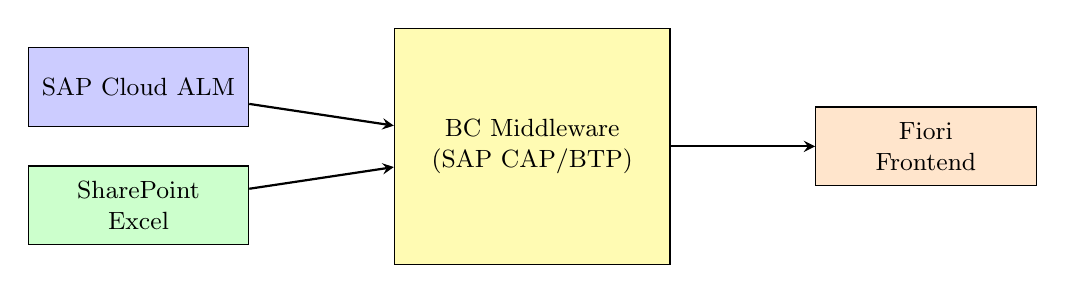
\begin{tikzpicture}[
    box/.style={rectangle, draw, minimum width=2.8cm, minimum height=1cm, align=center, font=\small},
    arrow/.style={->, >=stealth, thick}
]
    % Datenquellen links
    \node[box, fill=blue!20] (calm) at (0,1.5) {SAP Cloud ALM};
    \node[box, fill=green!20] (sharepoint) at (0,0) {SharePoint\\Excel};

    % Middleware Mitte
    \node[box, fill=yellow!30, minimum width=3.5cm, minimum height=3cm] (middleware) at (5,0.75) {BC Middleware\\(SAP CAP/BTP)};

    % Frontend rechts
    \node[box, fill=orange!20] (frontend) at (10,0.75) {Fiori\\Frontend};

    % Pfeile
    \draw[arrow] (calm) -- (middleware);
    \draw[arrow] (sharepoint) -- (middleware);
    \draw[arrow] (middleware) -- (frontend);
\end{tikzpicture}
\caption{Soll-Architektur der BC Middleware}
\label{fig:soll-architektur}
\end{figure}

Abbildung~\ref{fig:soll-architektur} zeigt die Zielarchitektur. Die zentrale Idee ist die Entkopplung des Frontends von der konkreten Datenquelle. Das Frontend kommuniziert ausschließlich mit der Middleware über eine standardisierte \gls{odata}-Schnittstelle. Die Middleware abstrahiert die Komplexität des Datenzugriffs und kann transparent zwischen Excel- und Service-Backend wechseln.

\subsection{Stakeholder-Analyse}

Für den erfolgreichen Entwurf der Middleware ist das Verständnis der beteiligten Stakeholder und ihrer Anforderungen essentiell \citep{sommerville2015}.

\begin{table}[H]
\centering
\caption{Stakeholder und ihre Interessen}
\label{tab:stakeholder}
\begin{tabularx}{\textwidth}{lXX}
\toprule
\textbf{Stakeholder} & \textbf{Rolle} & \textbf{Interesse} \\
\midrule
Projektleiter & Nutzt Budget-Reports für Entscheidungen & Aktuelle, korrekte Zahlen; einfache Bedienung \\
\midrule
Controller & Pflegt Budgetdaten und PSP-Zuordnungen & Effiziente Dateneingabe; Konsistenzprüfung \\
\midrule
Frontend-Entwickler & Entwickelt Fiori-Oberfläche & Stabile, dokumentierte API; OData-Konformität \\
\midrule
IT-Architekten & Plant zukünftige Integration & Austauschbarkeit; saubere Architektur \\
\midrule
SAP-Administratoren & Betreibt die Anwendung auf BTP & Einfaches Deployment; Monitoring \\
\bottomrule
\end{tabularx}
\end{table}

\subsection{Use Cases}

Die folgenden Use Cases beschreiben die wichtigsten Interaktionen mit dem System. Use Cases sind ein bewährtes Mittel der Anforderungsanalyse, um funktionale Anforderungen aus Nutzersicht zu dokumentieren \citep{sommerville2015}:

\subsubsection{UC-01: Budget-Übersicht abrufen}

\begin{table}[H]
\centering
\begin{tabularx}{\textwidth}{lX}
\toprule
\textbf{Akteur} & Projektleiter \\
\midrule
\textbf{Vorbedingung} & Benutzer hat Session gestartet \\
\midrule
\textbf{Ablauf} &
1. Benutzer öffnet Budget-Dashboard \\
& 2. Frontend ruft GET /BudgetOverview auf \\
& 3. Middleware lädt Excel, berechnet Metriken \\
& 4. Frontend zeigt Budget/Actual/ETC/EAC pro Team \\
\midrule
\textbf{Nachbedingung} & Aktuelle Budget-Metriken werden angezeigt \\
\bottomrule
\end{tabularx}
\caption{Use Case: Budget-Übersicht abrufen}
\end{table}

\subsubsection{UC-02: PSP-Zuordnung erstellen}

\begin{table}[H]
\centering
\begin{tabularx}{\textwidth}{lX}
\toprule
\textbf{Akteur} & Controller \\
\midrule
\textbf{Vorbedingung} & User Story existiert ohne PSP-Zuordnung \\
\midrule
\textbf{Ablauf} &
1. Controller wählt User Story aus Liste \\
& 2. Controller wählt PSP-Element aus Dropdown \\
& 3. Frontend ruft POST /createPSPAssignment auf \\
& 4. Middleware schreibt Zuordnung in Excel \\
& 5. Bestätigung wird angezeigt \\
\midrule
\textbf{Nachbedingung} & User Story ist PSP zugeordnet; ETC wird berechnet \\
\midrule
\textbf{Alternativ} & Bei Team-Mismatch: Warnung anzeigen \\
\bottomrule
\end{tabularx}
\caption{Use Case: PSP-Zuordnung erstellen}
\end{table}

\subsubsection{UC-03: Projekt wechseln}

\begin{table}[H]
\centering
\begin{tabularx}{\textwidth}{lX}
\toprule
\textbf{Akteur} & Alle Benutzer \\
\midrule
\textbf{Vorbedingung} & Mehrere Projekte sind konfiguriert \\
\midrule
\textbf{Ablauf} &
1. Benutzer ruft GET /getProjects() auf \\
& 2. Liste verfügbarer Projekte wird angezeigt \\
& 3. Benutzer wählt Projekt aus \\
& 4. POST /startSession mit Projektname \\
& 5. Session-ID wird zurückgegeben und gespeichert \\
\midrule
\textbf{Nachbedingung} & Alle folgenden Requests nutzen das gewählte Projekt \\
\bottomrule
\end{tabularx}
\caption{Use Case: Projekt wechseln}
\end{table}

\subsection{Anforderungsanalyse}

\subsubsection{Funktionale Anforderungen}

\begin{table}[H]
\centering
\caption{Funktionale Anforderungen}
\label{tab:fa}
\begin{tabularx}{\textwidth}{lX}
\toprule
\textbf{ID} & \textbf{Anforderung} \\
\midrule
FA-01 & Das System muss Budget-Metriken pro Team berechnen können \\
FA-02 & Das System muss Budget-Metriken pro \gls{psp} berechnen können \\
FA-03 & Das System muss \gls{crud}-Operationen für \gls{psp}-Zuordnungen unterstützen \\
FA-04 & Das System muss Session-basiertes Projekt-Management unterstützen \\
FA-05 & Das System muss Team-Mismatch-Warnungen generieren können \\
FA-06 & Das System muss Excel-Daten von SharePoint lesen können \\
FA-07 & Das System muss Änderungen zurück in Excel schreiben können \\
\bottomrule
\end{tabularx}
\end{table}

\subsubsection{Nicht-funktionale Anforderungen}

\begin{table}[H]
\centering
\caption{Nicht-funktionale Anforderungen}
\label{tab:nfa}
\begin{tabularx}{\textwidth}{lX}
\toprule
\textbf{ID} & \textbf{Anforderung} \\
\midrule
NFA-01 & Die Backend-Implementierung muss austauschbar sein \\
NFA-02 & Die \gls{api} muss \gls{odata} v4-kompatibel sein \\
NFA-03 & Das System muss auf der SAP \gls{btp} deploybar sein \\
NFA-04 & Die \gls{api} muss für ein Fiori-Frontend geeignet sein \\
NFA-05 & Das System muss ohne lokale Datenbankinstanz funktionieren \\
\bottomrule
\end{tabularx}
\end{table}

\subsection{Priorisierung der Anforderungen}

Die Anforderungen werden nach der MoSCoW-Methode priorisiert \citep{sommerville2015}:

\begin{table}[H]
\centering
\caption{Priorisierung der Anforderungen}
\label{tab:priorisierung}
\begin{tabularx}{\textwidth}{clX}
\toprule
\textbf{Prio} & \textbf{ID} & \textbf{Anforderung} \\
\midrule
\multirow{4}{*}{\textbf{Must}} & FA-01 & Budget-Metriken pro Team \\
& FA-02 & Budget-Metriken pro PSP \\
& FA-06 & Excel-Daten lesen \\
& NFA-02 & OData v4-kompatibel \\
\midrule
\multirow{3}{*}{\textbf{Should}} & FA-03 & CRUD für PSP-Zuordnungen \\
& FA-04 & Session-Management \\
& NFA-01 & Backend austauschbar \\
\midrule
\multirow{2}{*}{\textbf{Could}} & FA-05 & Team-Mismatch-Warnungen \\
& FA-07 & Excel Write-Back \\
\midrule
\textbf{Won't} & -- & Fiori-Frontend (andere Arbeit) \\
\bottomrule
\end{tabularx}
\end{table}

\subsection{Abgrenzung}

Folgende Aspekte sind nicht Bestandteil dieser Arbeit:
\begin{itemize}
    \item \textbf{Fiori-Frontend}: Die Benutzeroberfläche wird von anderen Studierenden im Rahmen separater Arbeiten entwickelt. Diese Arbeit stellt lediglich die API bereit.

    \item \textbf{Vollständige CALM-Integration}: Der OData-Adapter für SAP Cloud ALM wird konzeptionell beschrieben, aber nicht implementiert. Dies ermöglicht die Bewertung der Austauschbarkeit ohne vollständige Implementierung.

    \item \textbf{Benutzer-Authentifizierung}: Die Authentifizierung wird durch die SAP BTP (XSUAA Service) bereitgestellt und ist nicht Teil der Middleware-Implementierung.

    \item \textbf{Historisierung}: Eine vollständige Audit-Trail-Funktionalität für Änderungen ist nicht vorgesehen.

    \item \textbf{Mandantenfähigkeit}: Die Middleware unterstützt mehrere Projekte, aber keine vollständige Mandantentrennung mit separaten Datenbeständen.
\end{itemize}
